\documentclass[PST,authoryear,toc]{lsstdoc}
% lsstdoc documentation: https://lsst-texmf.lsst.io/lsstdoc.html

% Package imports go here.

% Local commands go here.

% To add a short-form title:
% \title[Short title]{Title}
\title{Understanding of  Telescope and Site Software situation}

% Optional subtitle
% \setDocSubtitle{A subtitle}

\author{%
William O'Mullane
}

\setDocRef{PSTN-002}

\date{\today}

% Optional: name of the document's curator
% \setDocCurator{The Curator of this Document}

\setDocAbstract{%
After several months with TSS these are some thoughts on the situation.
}

% Change history defined here.
% Order: oldest first.
% Fields: VERSION, DATE, DESCRIPTION, OWNER NAME.
% See LPM-51 for version number policy.
\setDocChangeRecord{%
  \addtohist{1}{YYYY-MM-DD}{Unreleased.}{William O'Mullane}
}

\begin{document}

% Create the title page.
% Table of contents is added automatically with the "toc" class option.

\mkshorttitle
%switch to \maketitle if you wan the title page and toc


% ADD CONTENT HERE ... a file per section can be good for editing

\section{Introduction} \label{sec:intro}
Having  been asked to look at Telescope and Site Software (TSS) after our review in Feb 2018  there are  one or two insights which should be shared. As we approach commissioning the focus of the team will change, there is no simple approach to this sort of system so we need to be open to the needs of commissioning.


\section{Code vs  Graphical Interface }

There are basic {\em truths} which we all hold {\em incorrectly} as empirical. I am a programmer I seldom touch a GUI unless I have to. I first saw this explained by Chris Beaumont in Vienna in 2014(\figref{fig:gspec}).
\begin{figure}
\begin{center}
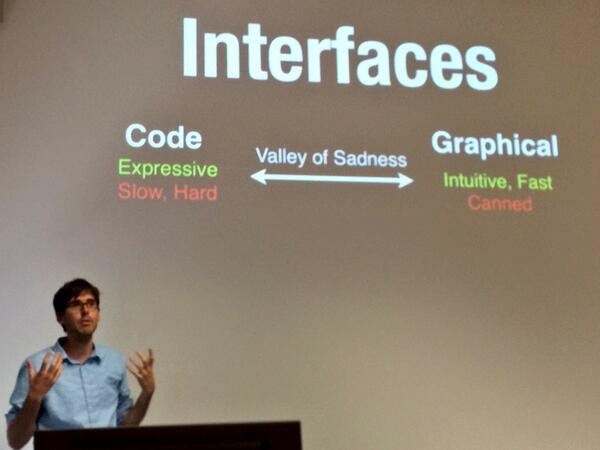
\includegraphics[width=0.6\textwidth]{beaumontCG}
\caption{Code and Graphics - Chris Beaumont Vienna 2014. \label{fig:gspec}}
\end{center}
\end{figure}

I had not thought much about this before but this talk crystallized it for me. I do make occasional plots and diagrams to explain things but it is not the norm. My mistake was to think all programmers are like this. Worse that all smart users were like this.
As with most things there is a spectrum as as in \figref{fig:gspec}, there are a range of approaches and people who use them.

TSS approach seems very graphical with an over  reliance on GUIs.
LabView, though it has scripting capability, is inherently graphical and many of us are biased against it\footnote{The license fees do not help}. It has good realtime multi threading capability and was certainly a viable choice for lower level control.
This may also be useful for commissioning but the commissioning team have not bought in to this mode of working.
 Looking at the OCS (Observatory Control System)  code this also assumes a GUI, every action like {\em StartNight} is assumed to be an action in a GUI\footnote{Actually it is assumed to be a state which is strictly true but semantically unclear. }.
There seems no way to call this from a script or command line. It seems naive to think we may be able to encapsulate this in a compiled routine\footnote{In Java} anytime before operations. There was certainly a need for engineering GUI's and some users request such things - but we need to take care that one approach does not suit all.


The LSST users, especially in commissioning, are highly efficient in abstract thinking, scripting and coding of one form or another. There has, perhaps,  been  a major misunderstanding of what users want from the control system. The TSS approach seems to be to provide canned high level procedures (right of \figref{fig:gspec}), the users want and need a much more open and flexible system.
The flexibility is totally necessary in commissioning. This may have been achievable with LabView scripting but the commissioning team have invested heavily in Python.
The canned approach is appropriate in later operations, but we have  a lot of AIT and commissioning to go through first.
Right now we do not know the list of procedures, even if we had the list we could not detail how to do them without going through commissioning - the first need is a scriptable system for commanding the observatory (left of \figref{fig:gspec}).


\section{Predicting State}
The second philosophical approach is toward state or the ability to know state. There is a basic principle in the TSS architecture that everything is  Finite State Machine (FSM).
Since the observatory is a series of machines this is strictly true, however we do not know all the possible states or modes of the machine(s)  and we probably will not know them until well into operations. For individual components
We will begin to learn this in commissioning. There has been a major conflict with  TSS team seeking the {\em requirements} from the T\&S team for several years.  LSST is complex and has some novel aspects, I believe TSS are looking for the full set of modes and states for LSST - I also believe it is impossible to know that for an as yet built system like LSST. Hence can one ever build an FSM for operations it before it is complete ?

The FSM is the {\em correct} approach  but it can not be applied system wide, i.e. at Telescope or Observatory level it is unclear this is the correct approach. We all fall in the trap of generalization.
In this case trying to apply the FSM approach to the entire system will never work and has locked the TSS team up in an impossible task -
the team has been waiting for the requirements (which define states)  while many of us understand we will not know those states until we are on the mountain with the actual hardware. This is not to suggest we should not have requirements, the level of detail we may get is not always sufficient plus we need to take care of over defining scope - we have to make the entire system work.

The FSM approach is inherently restrictive  it allows one to do exactly what is prescribed. A new observatory like LSST, especially in commissioning, needs a much more flexible and open approach. A very restrictive system with only {\em allowed} transitions often leads to ta situation where {\em the system} will not allow an activity even if the users/engineers/observatory scientist agree it is the correct action. Again this is probably ok in operations but not in commissioning.

For Example, at some point we will need to manipulate the louvers to control air flow.
 How we do that will depend on wind and temperatures - we do not know today how that will be done.
There will probably be some formula taking account of temperature inside the dome and airflow outside the dome.
Initially  we \footnote{The royal we here is really the commissioning team and operators.} will possibly adjust the louvers until we understand how they work over many nights, we may experiment with a number of formula looking at EFD and sending SAL commands. This of course can be built into a FSM using some algorithm selection.
 This requires a very flexible system,  not an FSM though of course once could make a more flexible FSM.

The above is an over simplification and a potential explanation for some of my observations.

\section{Way forward}
The Service Access Layer (SAL) gives a well defined interface to all components in the system no mater the implementing language.
We have constructed a Python component complying to this interface, this both allows us to quickly write a new component and to remote interact with any other component using Python. Hence this module gives scripting capability to the Telescope and Site Software with the full power of Python. An update to LSE-150, the TSS architecture, is underway to explain the current architecture, \figref{fig:sal} gives the high level SalObj view.


\begin{figure}
\begin{center}
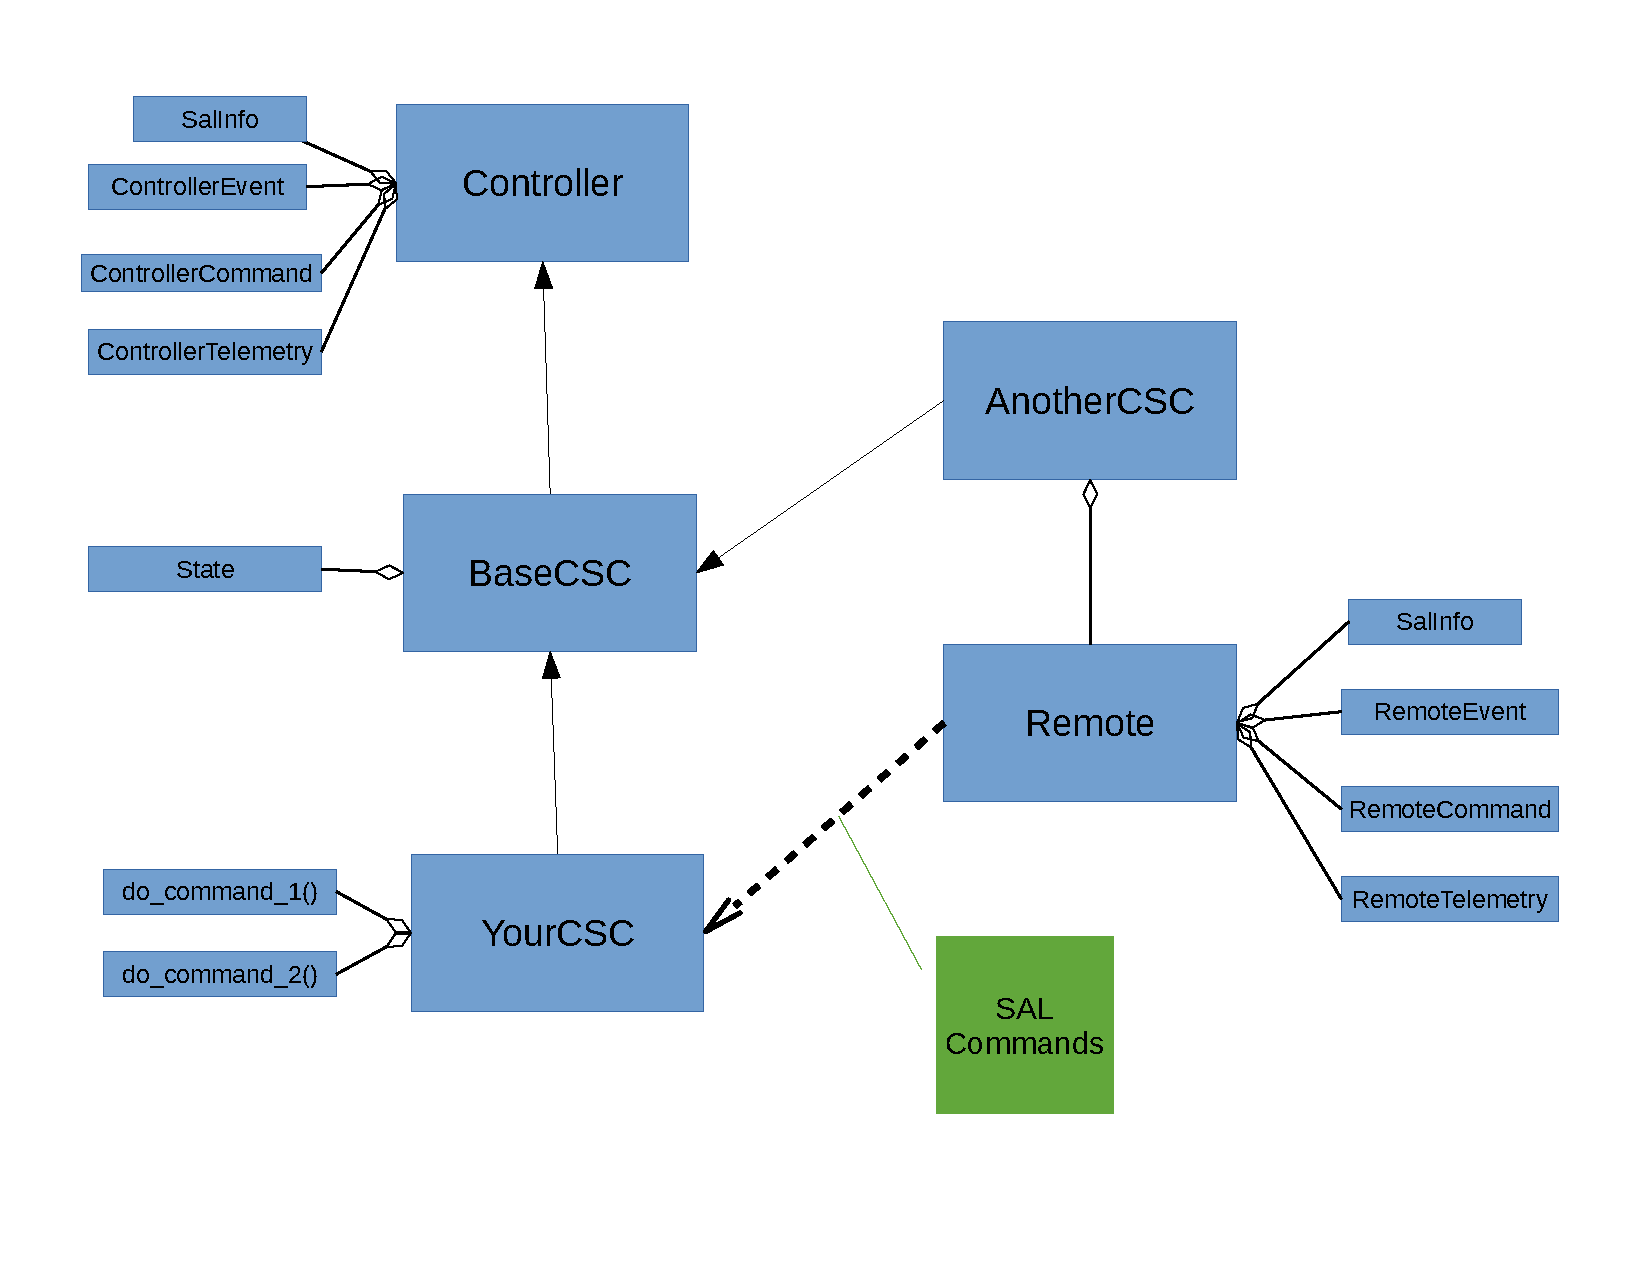
\includegraphics[width=0.6\textwidth]{SalobjClassDiag2}
\caption{SalObj is a Python module for implementing and interacting with Controllable SAL Components (CSCs) which allows for
flexible Python scripting. \label{fig:sal}}
\end{center}
\end{figure}


We are also addressing the planning in Primavera and Jira. We are starting with the approaching AuxTel milestones and building a plan to deliver the required components and environments to make that successfully.
We will concentrate on making individual components robust and building Python scripts to achieve high level coordination - less prominence will be placed on the control system components (ATCS, OCS, TCS)  for now.

There have been some management setbacks which are also being dealt with most recently by Andy Clements agreeing to be interim lead for  the team.

\section{Conclusion}
In TSS we need to focus on a flexible programmable interface to meet the  primary needs of AIT and commissioning.
Meanwhile we have an INRIA contract to build a graphical interface for Operations (and possibly some of commissioning).
This of this very much in the terms of hackable user interface \citep{2015ASPC..495..101B}.
We also do need to be aware of the safety of operating the system - as we build up scripts for testing, AIT and commissioning we will start to build more constraints into the system - we should not try to build all constraints in from the start.




\appendix
% Include all the relevant bib files.
% https://lsst-texmf.lsst.io/lsstdoc.html#bibliographies
\section{References} \label{sec:bib}
\renewcommand{\refname}{}
\bibliography{lsst,lsst-dm,refs_ads,refs,books}

%Make sure lsst-texmf/bin/generateAcronyms.py is in your path
\section{Acronyms used in this document}\label{sec:acronyms}
\addtocounter{table}{-1}
\begin{longtable}{|l|p{0.8\textwidth}|}\hline
\textbf{Acronym} & \textbf{Description}  \\\hline

AIT & Assembly, Integration, and Test \\\hline
EFD & Engineering Facilities Database \\\hline
FSM & Finite State Machine \\\hline
GUI & Graphical User Interface \\\hline
LSST & Large Synoptic Survey Telescope \\\hline
OCS & Observatory Control System \\\hline
PST & Project Science Team \\\hline
PSTN & Project Science Technical Note \\\hline
SAL & Service Access Layer \\\hline
T\&S & Telescope and Site \\\hline
TSS & Telescope and Site Software \\\hline
\end{longtable}

\end{document}
